\documentclass[12pt,addpoints]{evalua}
\grado{3$^\circ$ de Secundaria}
\cicloescolar{2023-2024}
\materia{Matemáticas 3 \normalfont \color{darkgray}\small con adecuación curricular a \\Matemáticas 6$^\circ$ de Primaria}
\unidad{1}
\title{Examen de la Unidad}
\aprendizajes{
      \item Resuelve problemas y operaciones con números naturales y fraccionarios.
      \item Comprende la ubicación de los números fraccionarios en la recta numérica.
      \item Conoce los difernetes tipos de fracciones y su representación gráfica.
      }

\author{Prof.: Julio César Melchor Pinto}
\begin{document}
\begin{questions}
    \section*{\ifprintanswers   {Sumas y restas}\else{}\fi}
    % \begin{multicols}{2}
    \subsection*{\ifprintanswers{Sumas}\else{}\fi}
    \question[10] Realiza las siguientes sumas:
    \begin{multicols}{2}
        \begin{parts}
            \part \large \opadd[resultstyle=\color{white},carryadd=false]{5892}{1084}
            \part \large \opadd[resultstyle=\color{white},carryadd=false]{243}{188}
        \end{parts}
    \end{multicols}

    \subsection*{\ifprintanswers{Restas}\else{}\fi}
    \question[8] Realiza las siguientes restas:
    \begin{multicols}{2}
        \begin{parts}
            \part \large \opsub[resultstyle=\color{white},carryadd=false]{1834}{1283}
            \part \large \opsub[resultstyle=\color{white},carryadd=false]{524}{89}
        \end{parts}
    \end{multicols}
    % \end{multicols}

    \subsection*{\ifprintanswers{Resolución de problemas}\else{}\fi}
    \question[10] Un consumidor de restaurante consumió \$230 pesos en comida, \$90 en bebidas y \$87 en postre. Si pagó con un billete de \$500 pesos, \textbf{¿cuánto cambio recibirá?}
    \begin{solutionbox}{2.5cm}
        Para saber cuánto cambio recibirá, se debe restar al billete de 500 pesos los productos consumidos, y lo que resulte será el cambio que recibirá; entonces: $500-230-90-87= 500-407=93$.
        Por lo tanto, recibirá \$93 pesos de cambio.
    \end{solutionbox}

    \question[10] Una editorial publica 12,000 libros de un autor y 10,560 libros de otro autor. ¿Cuántos libros en total publicó la editorial?
    \begin{solutionbox}{2.5cm}
        Para saber cuántos libros en total publicó la editorial, se deben sumar los libros de ambos autores; entonces: $12,000+10,560=22,560$.
        Por lo tanto, la editorial publicó 22,560 libros en total.
    \end{solutionbox}

    \section*{\ifprintanswers   {Multiplicaciones y divisiones}\else{}\fi}
    \begin{multicols}{2}
        \subsection*{\ifprintanswers{Multiplicaciones}\else{}\fi}
        \question[4] Realiza la siguiente multiplicación:
        \begin{multicols}{2}
            \begin{parts}
                \part \large\opmul[resultstyle=\color{white}\large,carryadd=false]{433}{8}
                % \part \opmul[resultstyle=\color{white},carryadd=false]{235}{155}
            \end{parts}
        \end{multicols}

        \subsection*{\ifprintanswers{Divisiones}\else{}\fi}

        \question[4] Realiza la siguiente división:
        \begin{multicols}{2}
            \begin{parts}
                \part \large\longdivision[stage=0]{175}{7}
                % \part \longdivision{0.0005}{0.5}
            \end{parts}
        \end{multicols}

    \end{multicols}

    \subsection*{\ifprintanswers{Resolución de problemas}\else{}\fi}
    \question[10] Resuelve los siguientes problemas:
    \begin{parts}
        \part Si un dólar equivale a \$19 pesos. ¿Cuántos pesos equivaldrán 615 dólares?
        \begin{solutionbox}{2.5cm}
            Para saber cuántos pesos equivaldrán 615 dólares, se debe multiplicar 615 por 19; entonces: $615\times 19=11,685$.
            Por lo tanto, 615 dólares equivalen a \$11,685 pesos.
        \end{solutionbox}

        \part Un tanque de gasolina se llena con 48 litros, si el costo por litro de gasolina es de \$21 pesos. ¿Cuánto se pagará para llenar el tanque?
        \begin{solutionbox}{2.5cm}
            Para saber cuánto se pagará para llenar el tanque, se debe multiplicar 48 por 21; entonces: $48\times 21=1,008$.
            Por lo tanto, se pagará \$1,008 pesos para llenar el tanque.
        \end{solutionbox}

    \end{parts}

    \section*{\ifprintanswers   {Introducción a fracciones}\else{}\fi}
    \subsection*{\ifprintanswers{Clasificación de fracciones}\else{}\fi}
    \question[10] Clasifica las siguientes fracciones en \textit{propias}, \textit{impropias} o \textit{mixtas}:
    \begin{multicols}{2}
        \begin{parts}
            \part $\dfrac{5}{6}=$ \fillin[Propia][1in]   \\
            \part $1\dfrac{5}{6}=$ \fillin[Mixta][1in]  \\
            \part $\dfrac{7}{6}=$ \fillin[Impropia][1in] \\
            % \part $\dfrac{3}{4}=$ \fillin[Propia][1in]   \\
            % \part $1\dfrac{2}{3}=$ \fillin[Mixta][1in]   \\
            \part $\dfrac{7}{5}=$ \fillin[Impropia][1in] \\
            \part $\dfrac{7}{8}=$ \fillin[Propia][1in] \\
            % \part $3\dfrac{2}{9}=$ \fillin[Mixta][1in]   \\
            % \part $\dfrac{3}{2}=$ \fillin[Impropia][1in]   \\
            % \part $4\dfrac{1}{4}=$ \fillin[Mixta][1in] \\
        \end{parts}
    \end{multicols}
    \subsection*{\ifprintanswers{Representación de fracciones}\else{}\fi}
    \question[10] Escribe sobre la línea la fracción que representa cada imagen:
    \begin{multicols}{2}
        \begin{parts}
            \part 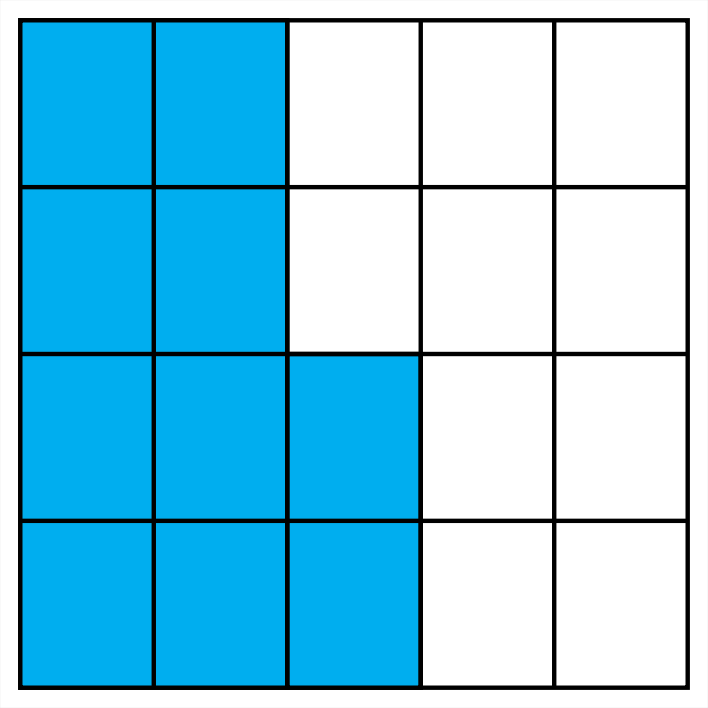
\includegraphics[width=70px]{../images/imagen_frac01.png} \fillin[$\dfrac{10}{20}$][1in]
            \part 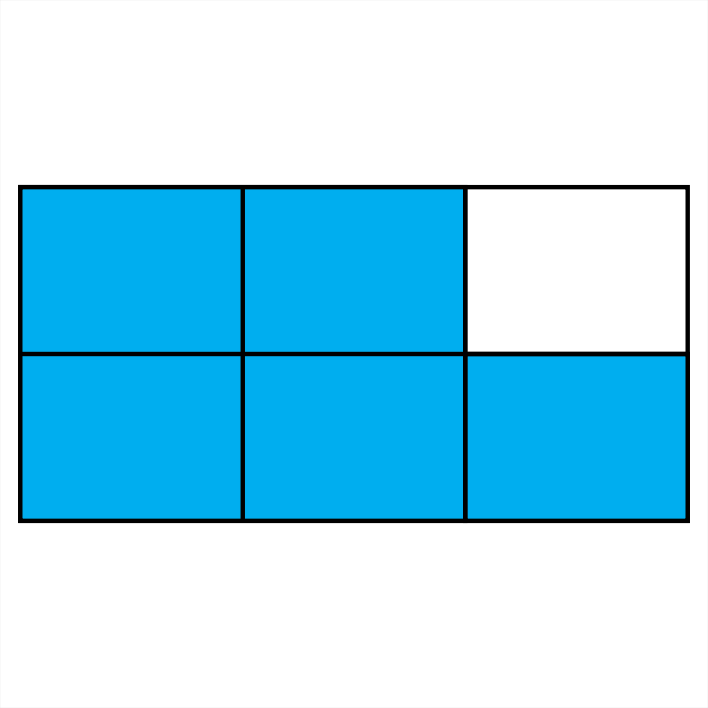
\includegraphics[width=70px]{../images/imagen_frac02.png} \fillin[$\dfrac{5}{6}$][1in]
            % \part 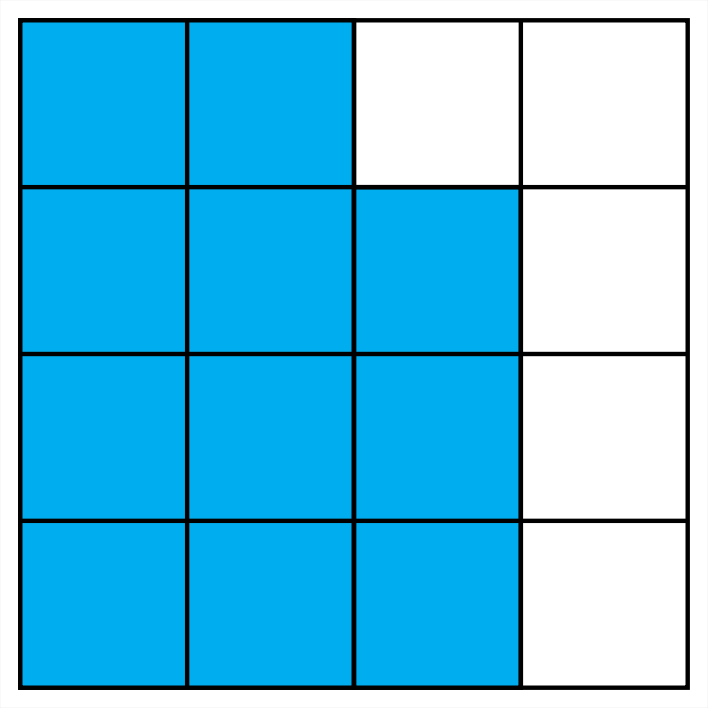
\includegraphics[width=100px]{../images/imagen_frac03.png} \fillin[$\dfrac{10}{20}$][1in]
            \part 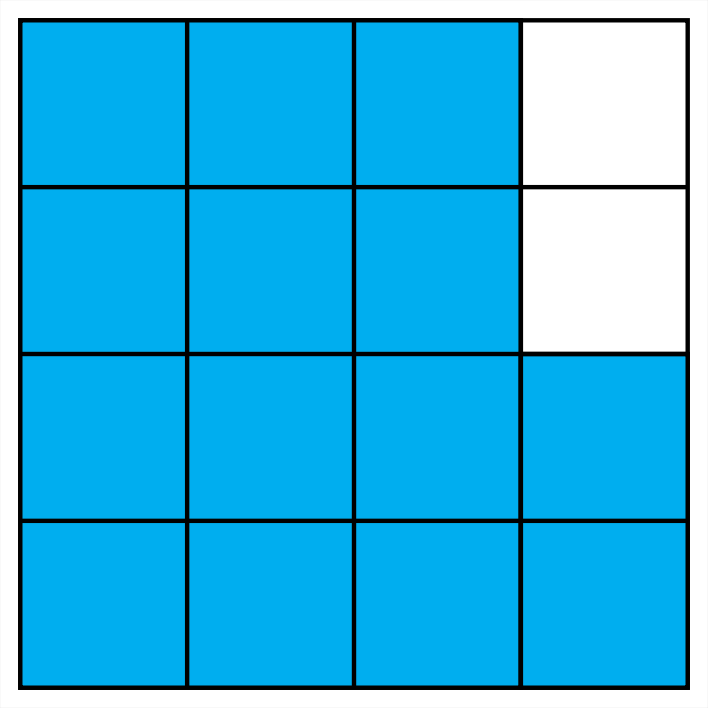
\includegraphics[width=70px]{../images/imagen_frac04.png} \fillin[$\dfrac{10}{20}$][1in]
            % \part 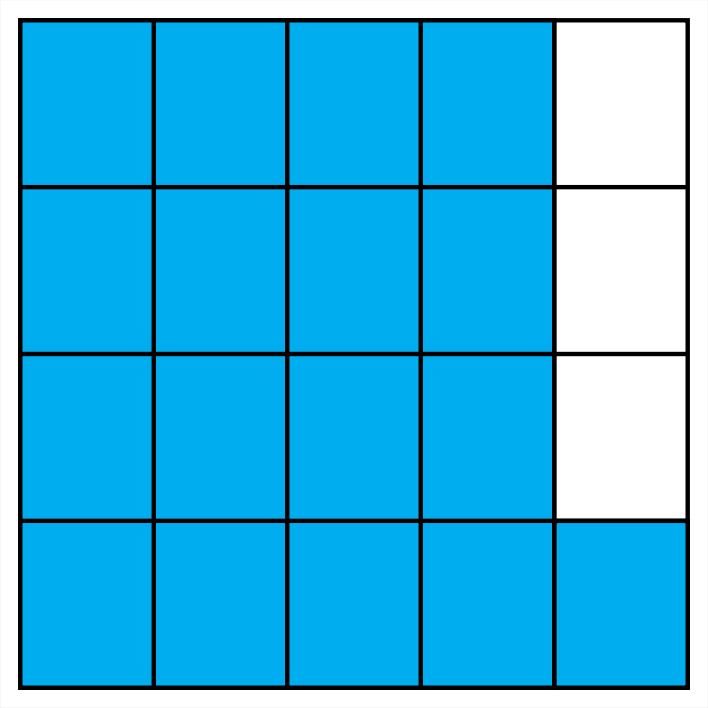
\includegraphics[width=100px]{../images/imagen_frac05.png} \fillin[$\dfrac{10}{20}$][1in]
            \part 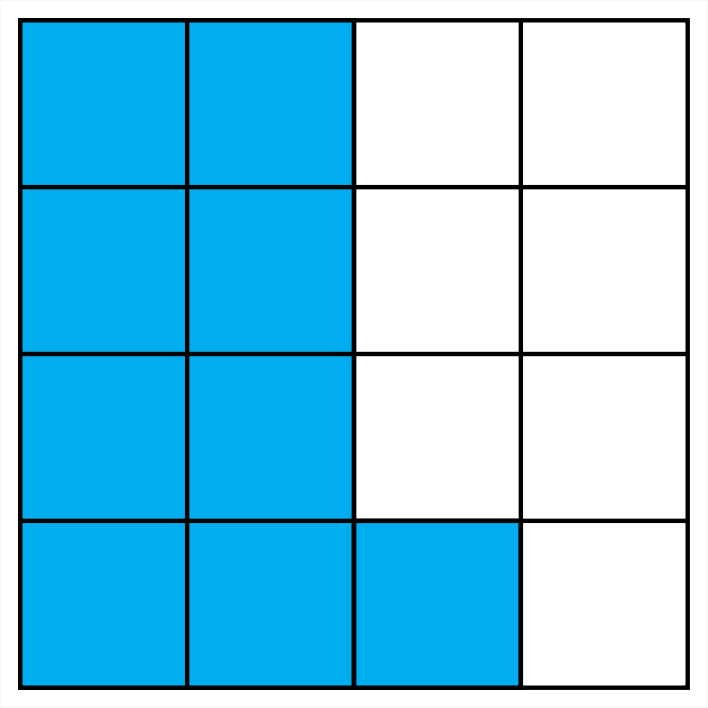
\includegraphics[width=70px]{../images/imagen_frac06.png} \fillin[$\dfrac{10}{20}$][1in]
            % \part 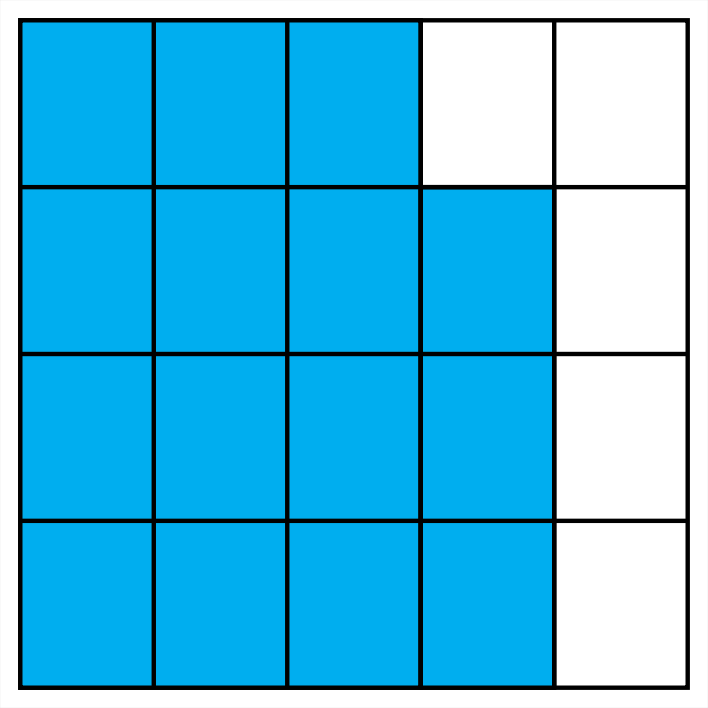
\includegraphics[width=100px]{../images/imagen_frac07.png} \fillin[$\dfrac{10}{20}$][1in]
            \part 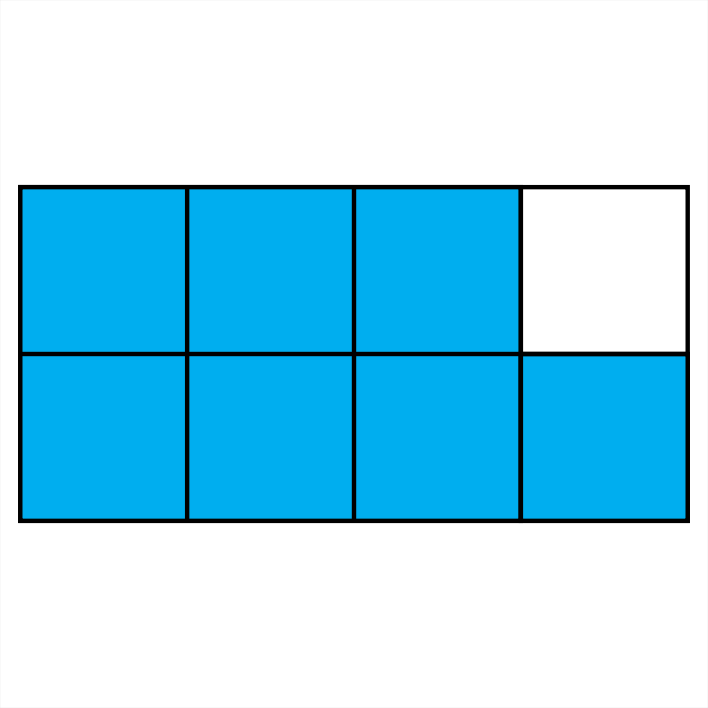
\includegraphics[width=70px]{../images/imagen_frac08.png} \fillin[$\dfrac{10}{20}$][1in]
            % \part 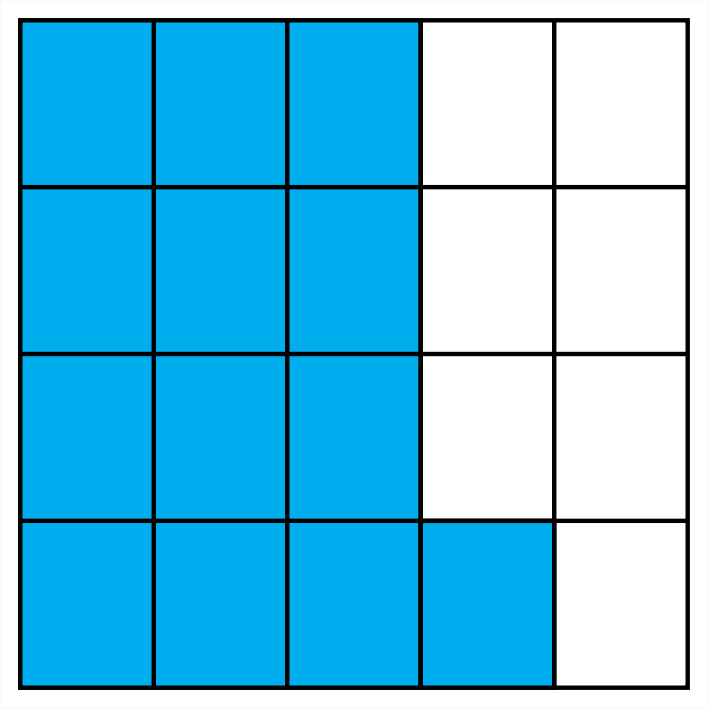
\includegraphics[width=100px]{../images/imagen_frac09.png} \fillin[$\dfrac{10}{20}$][1in]
            \part 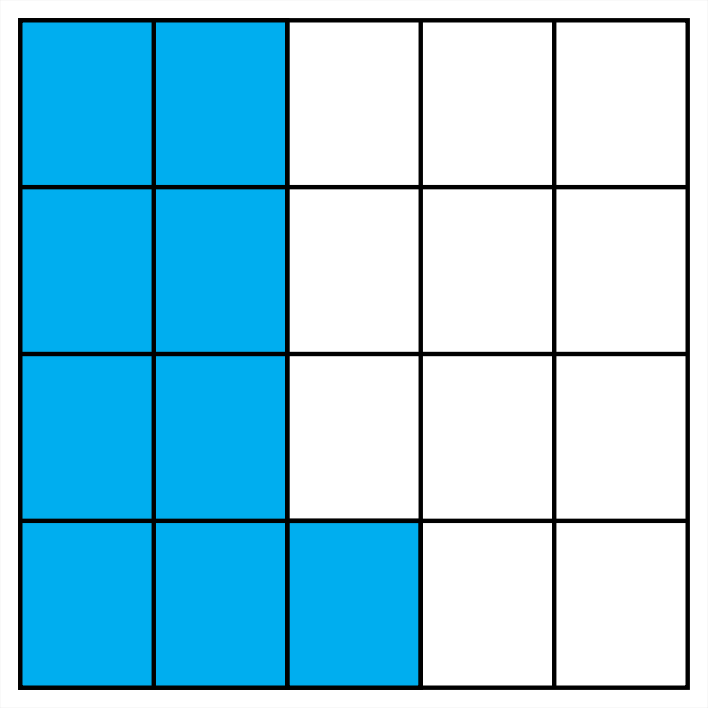
\includegraphics[width=70px]{../images/imagen_frac10.png} \fillin[$\dfrac{10}{20}$][1in]
        \end{parts}
    \end{multicols}

    \subsection*{\ifprintanswers{Nombre de fracciones}\else{}\fi}

    \question[8] Escribe la fracción que corresponda en cada inciso:

    \begin{parts}
        % \part ¿Cómo se escribe numéricamente la fracción \textbf{ocho quintos}?    \fillin[$\dfrac{8}{5}$][0in]  \\
        \part ¿Cómo se escribe numéricamente la fracción \textbf{seis onceavos}?   \fillin[$\dfrac{6}{11}$][0in]

        % \begin{solutionbox}{1cm}\small
        %     La fracción se lee como \textit{seis onceavos} y se escribe como $\dfrac{6}{11}$.
        % \end{solutionbox}
        % \part ¿Cómo se escribe numéricamente la fracción \textbf{dos séptimos}?    \fillin[$\dfrac{2}{7}$][0in]  \\

        \part ¿Cómo se escribe numéricamente la fracción \textbf{once medios}?     \fillin[$\dfrac{11}{2}$][0in]

        % \begin{solutionbox}{1cm}\small
        %     La frase \textit{once medios} se escribe como $\dfrac{11}{2}$.
        % \end{solutionbox}

        % \part ¿Cómo se escribe numéricamente la fracción \textbf{diez décimos}?    \fillin[$\dfrac{10}{10}$][0in]\\
    \end{parts}

    \subsection*{\ifprintanswers{Fracciones en la recta numérica}\else{}\fi}

    \question[8] Escribe la fracción que representa el punto en la recta numérica
    \begin{multicols}{2}
        \begin{parts}
            \part 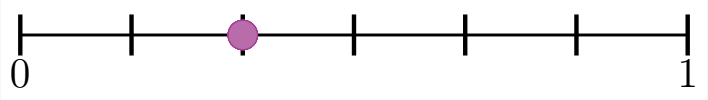
\includegraphics[width=150px]{../images/recta_num_frac01.png} \\[-0.5em] \fillin[$\dfrac{2}{6}$][2in]
            \part 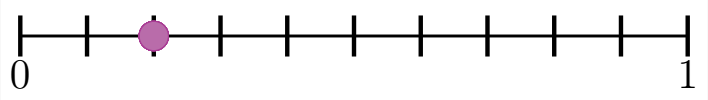
\includegraphics[width=150px]{../images/recta_num_frac02.png} \\[-0.5em] \fillin[$\dfrac{2}{10}$][2in]
            % \part 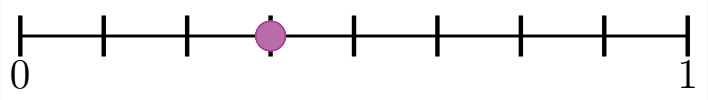
\includegraphics[width=150px]{../images/recta_num_frac03.png} \\[-0.5em] \fillin[$\dfrac{2}{6}$][1.5in]
            % \part 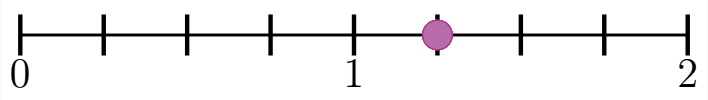
\includegraphics[width=150px]{../images/recta_num_frac04.png} \\[-0.5em] \fillin[$\dfrac{2}{6}$][1.5in]
            % \part 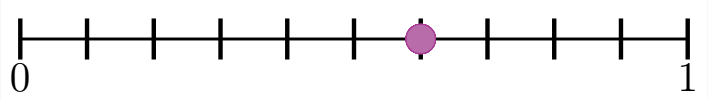
\includegraphics[width=150px]{../images/recta_num_frac05.png} \\[-0.5em] \fillin[$\dfrac{2}{6}$][1.5in]
            % \part 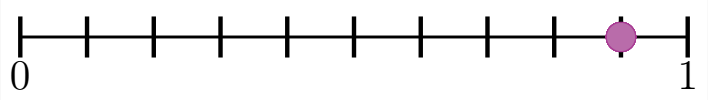
\includegraphics[width=150px]{../images/recta_num_frac06.png} \\[-0.5em] \fillin[$\dfrac{2}{6}$][1.5in]
            % \part 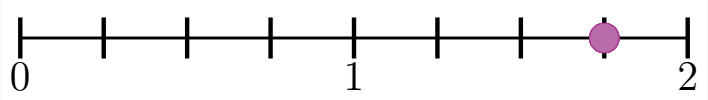
\includegraphics[width=150px]{../images/recta_num_frac07.png} \\[-0.5em] \fillin[$\dfrac{2}{6}$][1.5in]
            % \part 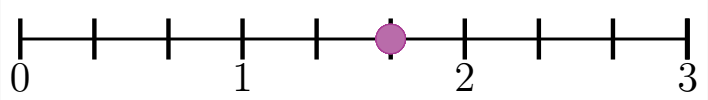
\includegraphics[width=150px]{../images/recta_num_frac08.png} \\[-0.5em] \fillin[$\dfrac{2}{6}$][1.5in]
            % \part 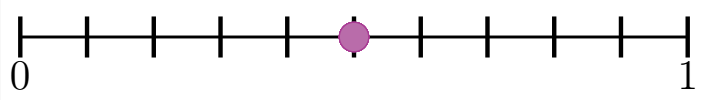
\includegraphics[width=150px]{../images/recta_num_frac09.png} \\[-0.5em] \fillin[$\dfrac{2}{6}$][1.5in]
            % \part 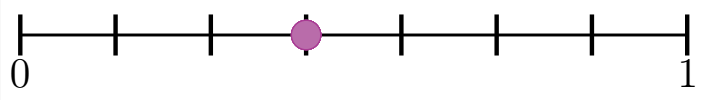
\includegraphics[width=150px]{../images/recta_num_frac10.png} \\[-0.5em] \fillin[$\dfrac{2}{6}$][1.5in]
        \end{parts}
    \end{multicols}

    \subsection*{\ifprintanswers{Conversión de fracciones}\else{}\fi}

    \question[8] Convierte las siguientes fracciones impropias a mixtas y viceversa:
    \begin{multicols}{3}
        \begin{parts}
            \part $\dfrac{17}{2}= $ \fillin[$8\dfrac{1}{2}$][0in]
            % \part $\dfrac{63}{10}= $ \fillin[$6\dfrac{3}{10}$][0in]
            \part $4\dfrac{1}{5}= $ \fillin[$\dfrac{21}{5}$][0in]
        \end{parts}
    \end{multicols}
\end{questions}
\end{document}